\section{GraphMAE算法原理}\label{sec:method}
\subsection{问题定义与整体信息流}
设无向属性图为$G=(V,E,X)$，$N=|V|$为节点数，$A\in\{0,1\}^{N\times N}$为邻接矩阵，$X\in\mathbb R^{N\times F}$为节点特征矩阵，$x_i\in\mathbb R^F$表示第$i$个节点的特征向量。预训练不使用类别标签，目标是学习编码器$f_E$，使其表示可支持少量标注下的节点分类。图\ref{fig:graphmae}展示官方流程。后文公式采用列向量描述单个节点，用矩阵的行堆叠表示整图。

\begin{figure}[tbp]
\centering
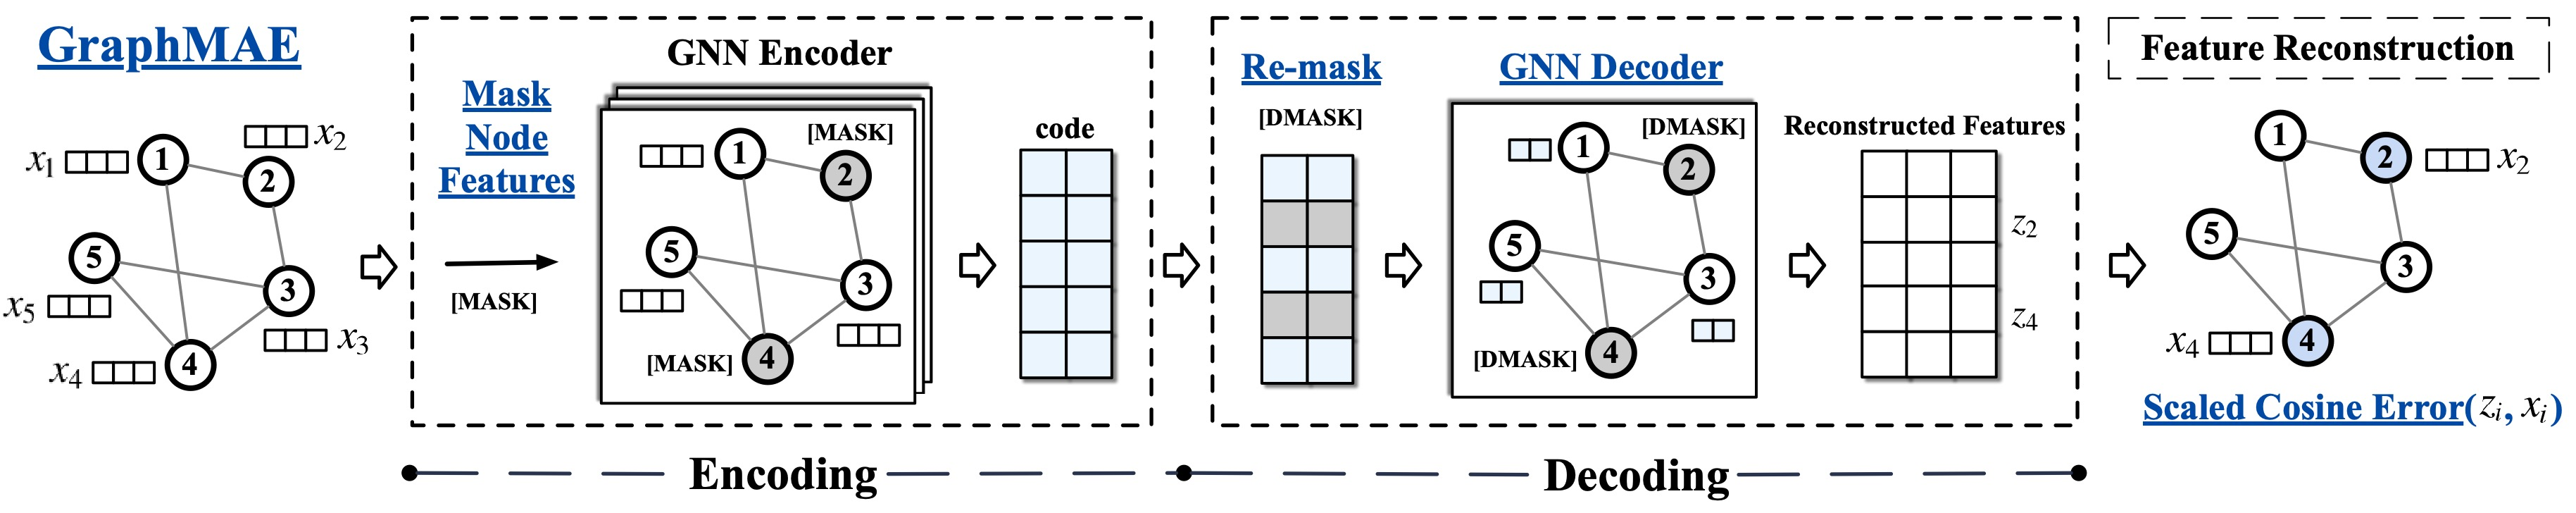
\includegraphics[width=\linewidth]{figures/graphmae_official.jpg}
\caption{GraphMAE整体流程。图片直接取自官方仓库，内容对应原论文图2中的GraphMAE部分\cite{hou2022graphmae}，并非本文新设计的架构。输入特征经掩码、GNN编码、重掩码与GNN解码后，在被选节点上计算SCE。锁定Cora实现中重掩码使用零向量。}
\label{fig:graphmae}
\end{figure}

模型的输入是图结构及部分可见特征，输出是重建特征$Z\in\mathbb R^{N\times F}$。本文计算图采用先去自环、再逐节点加一次自环的邻接关系$\bar A$。结构用于编码和解码的邻域聚合，并未作为预测目标引入边重建损失。

\subsection{节点特征掩码与随机替换}
设掩码比例为$r$，原始策略每轮均匀、无放回选择集合$M$：
\begin{equation}\label{eq:uniform}
k=\lfloor rN\rfloor,\quad M\subset V,\quad |M|=k,\qquad
M\sim\operatorname{UniformWithoutReplacement}(V,k).
\end{equation}
各节点的边际纳入概率为$k/N$。这里遮蔽的是节点特征，节点及关联边仍保留，故编码器可沿图结构传播信息。对Cora，$N=2708,r=0.5$，每轮选择1354个不同节点。

原论文的基本描述是用可学习向量$x_{\rm mask}$替换选中节点特征。实际配置还对少量选中节点随机替换为其他节点特征，以缓和预训练与无掩码推断的差异。设$T\subset M$为mask token节点、$R\subset M$为随机替换节点，$T\cap R=\varnothing$，则
\begin{equation}\label{eq:corruption}
\widetilde x_i=\begin{cases}
x_{\rm mask},& i\in T,\\
x_{j(i)},& i\in R,\\
x_i,& \text{其他},
\end{cases}
\end{equation}
其中$j(i)$为随机选取的特征供体节点，$x_{\rm mask}\in\mathbb R^F$初始为零并参加梯度更新。锁定源码分别计算$|T|=\lfloor(1-q)k\rfloor$和$|R|=\lfloor qk\rfloor$，$q=0.05$。因此1354个选中节点中1286个使用token，67个随机替换，另1个因两次取整而保留原特征；它仍属于$M$，参加后续重掩码与损失计算。本文保留这一实现细节，没有将其改成新的扰动比例。

\subsection{GAT编码器}
编码器计算$H=f_E(\bar A,\widetilde X)$。令$h_i^{(l)}$为第$l$层节点表示，初值$h_i^{(0)}=\widetilde x_i$；第$a$个注意力头采用投影矩阵$W^{(l,a)}$和源、目标注意力向量$u_{\rm src}^{(l,a)},u_{\rm dst}^{(l,a)}$。省略Dropout时，边$j\to i$的打分和邻域归一化为
\begin{align}
e_{ij}^{(l,a)}&=\operatorname{LeakyReLU}\!\left[
(u_{\rm dst}^{(l,a)})^{\mathsf T}W^{(l,a)}h_i^{(l)}+
(u_{\rm src}^{(l,a)})^{\mathsf T}W^{(l,a)}h_j^{(l)}\right],\label{eq:attention-score}\\
\beta_{ij}^{(l,a)}&=\frac{\exp(e_{ij}^{(l,a)})}
{\sum_{v\in\mathcal N(i)\cup\{i\}}\exp(e_{iv}^{(l,a)})}.\label{eq:attention-weight}
\end{align}
邻域$\mathcal N(i)$不含节点自身，额外的$\{i\}$对应自环。用$K$个头拼接并加入偏置，可写出层更新：
\begin{equation}\label{eq:gat-update}
h_i^{(l+1)}=\sigma\!\left[
\mathop{\Vert}_{a=1}^{K}\left(\sum_{j\in\mathcal N(i)\cup\{i\}}
\beta_{ij}^{(l,a)}W^{(l,a)}h_j^{(l)}\right)+b^{(l)}\right].
\end{equation}
符号$\Vert$表示拼接，$b^{(l)}$为拼接后的偏置，$\sigma$为激活函数。训练时每层投影前对输入特征做Dropout，softmax后对注意力系数做Dropout；此时实际用于聚合的系数不必再严格和为1。Cora编码器使用两层GAT，每层4头、每头128维，总输出512维，激活为PReLU；特征与注意力Dropout分别为0.2、0.1，LeakyReLU斜率0.2，不使用残差和归一化层。式\eqref{eq:attention-score}--\eqref{eq:gat-update}对应官方自定义PyG消息传递实现，而非任意默认配置的GAT模块。

\subsection{线性映射、Re-mask与解码器}
编码后先用无偏置线性层将表示映射到解码输入空间，再将同一个$M$内节点的表示置零：
\begin{equation}\label{eq:remask}
H=f_E(\bar A,\widetilde X),\quad Q=HW_{ED},\qquad
\widetilde q_i=\begin{cases}0,&i\in M,\\q_i,&i\notin M,\end{cases}
\quad Z=f_D(\bar A,\widetilde Q).
\end{equation}
其中$W_{ED}\in\mathbb R^{512\times512}$，$H,Q,\widetilde Q\in\mathbb R^{N\times512}$。原论文以解码掩码token描述Re-mask，式\eqref{eq:remask}按本次锁定源码具体写为零向量。它阻止解码器直接读取被掩码节点自身的编码表示，促使其借助邻居恢复特征；但邻居编码已融合过局部信息，因此不能理解为消除了所有关于这些节点的间接信号。

解码器是一层GAT，以1个输出头恢复$F=1433$维特征，最后一层不使用编码器的PReLU激活。其结构在本次Cora实现中固定，不随编码器两层设置而变成两层。表\ref{tab:dimensions}给出张量维度。下游推断只保留编码器，不使用投影层、Re-mask或解码器。
\begin{table}[tbp]
\centering\small
\caption{Cora路径中的主要张量与模块维度。}\label{tab:dimensions}
\begin{tabular}{lll}\toprule
对象/模块 & 输入 & 输出\\\midrule
掩码前后特征$X,\widetilde X$ & $2708\times1433$ & $2708\times1433$\\
GAT编码第1层 & $2708\times1433$ & $2708\times(4\times128)$\\
GAT编码第2层 & $2708\times512$ & $2708\times(4\times128)$\\
无偏置投影与Re-mask & $2708\times512$ & $2708\times512$\\
单层GAT解码器 & $2708\times512$ & $2708\times(1\times1433)$\\
下游线性分类器 & $2708\times512$ & $2708\times7$\\\bottomrule
\end{tabular}
\end{table}

\subsection{缩放余弦误差}
原论文提出缩放余弦误差（Scaled Cosine Error，SCE）作为特征恢复目标。令$z_i$为重建向量，$\gamma\ge1$为缩放指数，损失只在$M$上计算：
\begin{equation}\label{eq:sce}
\mathcal L_{\rm SCE}=\frac1{|M|}\sum_{i\in M}
\left(1-\frac{x_i^{\mathsf T}z_i}{\|x_i\|_2\|z_i\|_2}\right)^\gamma.
\end{equation}
该式对应原论文式(2)。实现先沿特征维做$\ell_2$归一化，范数分母使用epsilon保护，再计算余弦误差的幂及均值。与直接MSE相比，归一化减弱向量尺度对目标的影响；当余弦误差小于1时，较大的指数会更快降低易例的贡献，但不能据此声称所有误差均被缩小。Cora设$\gamma=3$，代码参数名为\texttt{alpha\_l}，与后文采样指数$\alpha_d$无关。

\subsection{预训练与冻结线性评估}
预训练以全图特征扰动后的SCE优化编码器、投影、解码器和mask token，不接收类别标签。完成后用无掩码特征生成冻结表示$U=f_E(\bar A,X)\in\mathbb R^{N\times512}$。线性分类器以$W_c\in\mathbb R^{512\times C}$及偏置$b_c\in\mathbb R^C$产生类别概率：
\begin{equation}\label{eq:classifier}
P=\operatorname{softmax}(UW_c+\mathbf1 b_c^{\mathsf T}),\qquad
\mathcal L_{\rm cls}=-\frac1{|V_{\rm tr}|}\sum_{i\in V_{\rm tr}}\log P_{i,y_i}.
\end{equation}
$C=7$，$y_i$为训练标签，$V_{\rm tr}$为训练节点集；实现中交叉熵直接接受logits，不显式先做softmax。encoder在这一阶段不更新。最终Probe完整训练300轮后，按验证准确率选择分类器：
\begin{equation}\label{eq:probe-selection}
t^*=\max\arg\max_{1\le t\le300}\operatorname{Acc}_{\rm val}(t).
\end{equation}
外层$\max$表示验证平分时保留较晚轮，与官方\texttt{>=}规则一致。测试标签仅在选模完成后用于最终评分；具体预训练和周期Probe协议见第\ref{sec:protocol}节。
